\documentclass[11pt, a4paper,twocolumn]{jarticle}
\usepackage[dvipdfmx]{graphicx}
\usepackage{listings,jlisting}
\usepackage{amssymb}
\usepackage{docmute}
\begin{document}
\begin{titlepage}
  \begin{center}
    {\Huge G.レーザートラッピング}\\
    \vspace{30truept}
    {\huge   提出者 : 08A17153 羽田充宏}\\ % 学籍番号
    {\huge 共同実験者 : 08A17179 牧野将之}\\
    {\huge       : 08A17205 森本拓実}\\ % 学籍番号
    \vspace{50truept}

    \begin{list}{}{\setlength{\leftmargin}{95pt}}
    \item {\huge 実験実施日 : 2019年12月2日}\\
    \vspace{10truept}
    \item {\huge 実験実施日 : 2019年12月9日}\\
    \vspace{10truept}
    \item {\huge 実験実施日 : 2019年12月16日}\\
    \vspace{10truept}
    \item {\huge 実験実施日 : 2019年12月23日}\\
    \vspace{10truept}
    \item {\huge 実験実施日 : 2020年1月6日}\\
    \vspace{10truept}
    \item {\huge 実験実施日 : 2020年1月20日}\\
    \vspace{40truept}

    \end{list}
    \vspace{50truept}

  \end{center}
\end{titlepage}


% template======================================================
% \section{}
% \subsection{}
% \subsubsection{Purpose}
% \subsection{Equipment}
% \begin{itemize}
%     \item
% \end{itemize}
% \subsubsection{Procedure}
% \subsubsection{Result}
% \subsubsection{Discussion}
%=============================================================
% \begin{figure}[ht]
%  \begin{center}
%   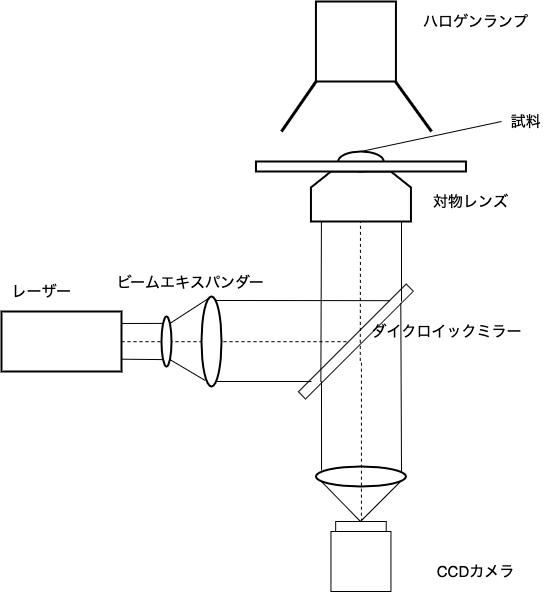
\includegraphics[width=0.8\linewidth]{fig1.png}
%  \end{center}
%  \caption{74HC14}
%  \label{fig:1}
% \end{figure}
% \clearpage
%=============================================================
\twocolumn
[
\begin{center}
    \textbf{\Large 実験目的}\\
    \begin{flushleft}
        \begin{itemize}
            \item 光学顕微鏡の取り扱い方法を身に付ける.
            \item 光の放射圧について理解し,レーザートラッピングの原理を理解する.
            \item 溶媒の粘性と粒子の運動について理解する.
        \end{itemize}
    \end{flushleft}
    \textbf{\Large 使用する実験器具}\\
    \begin{flushleft}
        \textbf{光学装置}
        \begin{itemize}
            \item 光学顕微鏡(ニコン倒立顕微鏡 TE-2000S)
            \item Nd:YAGレーザー(DPGL-2150F Photop Suwtech,Inc. 波長532nm,出力160W)
            \item 対物レンズ(浸水,NA1.15,倍率$\times$40)
            \item 対物レンズ(NA0.95,倍率$\times$60)
            \item ビームエキスパンダー
            \item ビームステアリング
            \item ミラー
        \end{itemize}
        \textbf{画像機器}
        \begin{itemize}
            \item CCDカメラ
            \item テレビモニター
        \end{itemize}
        \textbf{ステージ}
        \begin{itemize}
            \item XY軸ステッピングモーター(UG0348 駿河精機,4nm/pps)
        \end{itemize}
        \textbf{資料}
        \begin{itemize}
            \item 微粒子:ポリスチレン球(直径:0.5-10$\mu$m)
            \item ガラスボトムティッシュ
            \item サンプル管
            \item 純水
            \item 界面活性剤
            \item スポイト
        \end{itemize}
    \end{flushleft}
\end{center}
\vspace{30truept}
]
%=============================================================
 \documentclass[11pt, a4paper,twocolumn]{jarticle}
\usepackage[dvipdfmx]{graphicx}
\begin{document}
%=============================================================
\section{光学系の構築 (1日目)}
\subsection{実験目的}
今回の実験目的は光学系のアライメントを正確に行うことと,構築した光学系を用いてビーズのトラッピングを行うことである.

\subsection{実験手順}
まずダイヤルを回して出力電流を変えることでレーザー光の強さを調節した.
次にミラーを2枚用いてレーザー光を光学顕微鏡へ導入し,顕微鏡後側と対物レンズリボルバーに貼り付けられた的の真ん中にレーザー光が通過するようにミラーの位置と角度を調節した.
次にステージにスライドガラスを置いた後,リボルバーに水浸対物レンズを装着し,その上に蒸留水を2滴垂らした.またこのとき補正環は0.17に設定した.
さらに顕微鏡に入射した光がダイクロイックミラーによって試料ステージに反射されるように設定した.
その後CCDカメラによってレーザーがスライドガラス上に集光されることを確認した.
同心円状に集光できているかを確認し,モニターで映し出される集光スポットの中心にシールで目印を付けた.
次にミラーと顕微鏡の間にビームエキスパンダーを挿入し,同心円状に集光するまでビームエキスパンダーの位置の調整を行った.
完成した光学系は図\ref{fig:1}のようになった.

\begin{figure}[htbp]
 \begin{center}
  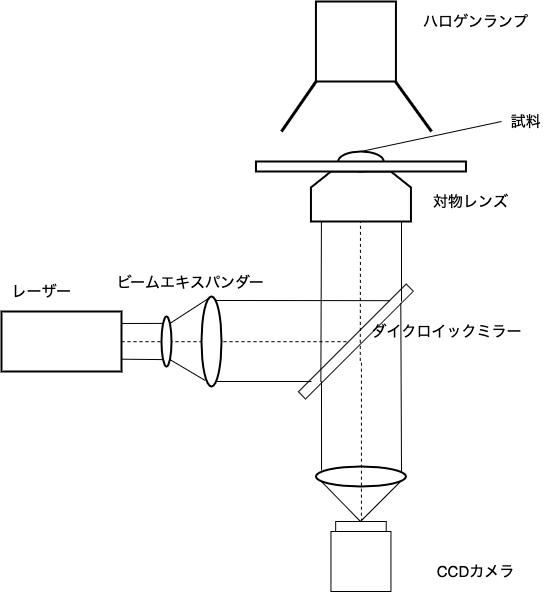
\includegraphics[width=0.8\linewidth]{fig1.png}
 \end{center}
 \caption{実験の光学系}
 \label{fig:1}
\end{figure}

\begin{figure}[htbp]
 \begin{center}
  \includegraphics[width=0.8\linewidth]{fig1-1.png}
 \end{center}
 \caption{同心円状パターン}
 \label{fig:1-1}
\end{figure}

\subsection{結果}
光学系の調整を行った図\ref{fig:1-1}のような同心円状の集光パターンが得られた.
また対物レンズの位置をスライドガラスを置いた試料ステージに近づけていくと2箇所で集光した.



\subsection{考察}
まずビームエキスパンダーを設置した理由について考察する.
レザー光は凸レンズに入射する事で一点に集光するがある程度の広がりを持つ.この時のスポット径を$d_0$,レンズの焦点距離f,レーザー波長$\lambda$,開口の直径をD,媒質の屈折率をnとすると以下の式で表せる.
\begin{equation}
    d = \frac{1.22f\lambda}{nD}
\end{equation}
よってビームエキスパンダーによってDの値を大きくする事でより集光スポットを小さくする目的があると考えられる.

さらに水侵対物レンズを用いる理由は対物レンズを抜けた光が進む媒質を水(n=1.33)にすることで集光スポット径をさらに小さくするためだと考えられる.

顕微鏡に入射した光をダイクロイックミラーで反射させたのは,ダイクロイックミラーが523nm以下の波長の光を透過して,それ以上の波長の光を反射させる性質を利用して,スライドガラスに反射したレザー光によって試料が観測できなくなる事を防ぐ目的であると考えられる.

また,光学顕微鏡へレーザー光を導入するときにミラーを2枚使った理由は任意の座標に任意の方向から光を入射させるためにはミラーが2枚必要であるからだと考えられる.

集光した際に図\ref{fig:1-1}のような同心円状パターンが得られた理由は対物レンズで集光した際にレンズの外側を通過する光と内側を通過する光で光路差が異なるために干渉をおこしレンズ中心からの距離に応じて明線,暗線が生じたためだと考えられる.

%=============================================================
\newpage
\end{document}

\documentclass[11pt, a4paper,twocolumn]{jarticle}
\usepackage[dvipdfmx]{graphicx}
\usepackage{listings,jlisting}

\begin{document}
%=============================================================
\section{Measure of the resistivity($2^{nd} day$)}

\subsection{Purpose}
金属の電流電圧特性を測定する.
\subsection{Procedure}
4端子測定法により以下に示す試料の抵抗を求める.
測定した抵抗値から試料の長さ,直径を考慮してそれぞれの試料の抵抗率を求める.
また今回の測定は全てl = 1cmの幅で行った.
\begin{itemize}
    \item A copper wire
    \item A NiCr wire
    \item A tungsten wire
    \item A lead of automatic pencil(H,2B)
    \item A Ni wire
    \item An Ag wire
    \item An unknown sample
\end{itemize}
\subsection{Result}
測定の結果電流電圧の関係をプロットすると以下のようなグラフが得られた.

\begin{figure}[htbp]
 \begin{center}
  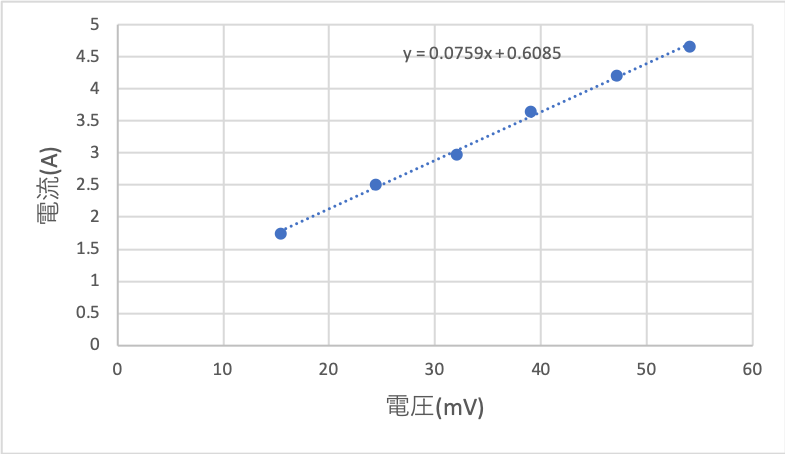
\includegraphics[width=0.8\linewidth]{fig15.png}
 \end{center}
 \caption{Cu}
 \label{fig:15}
\end{figure}

\begin{figure}[htbp]
 \begin{center}
  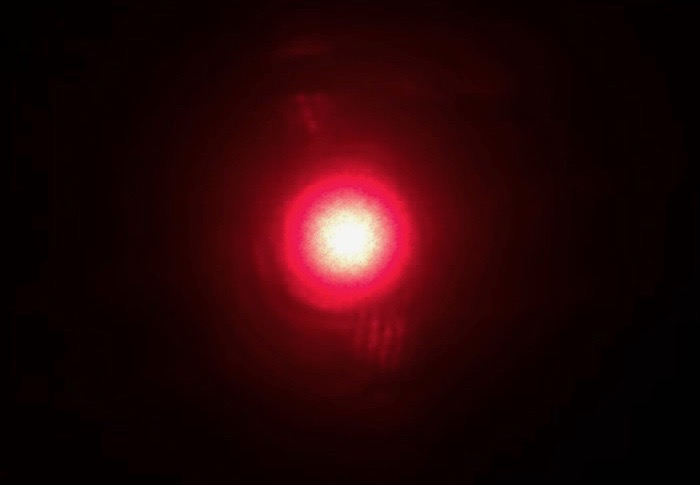
\includegraphics[width=0.8\linewidth]{fig16.png}
 \end{center}
 \caption{NiCr}
 \label{fig:16}
\end{figure}

\begin{figure}[htbp]
 \begin{center}
  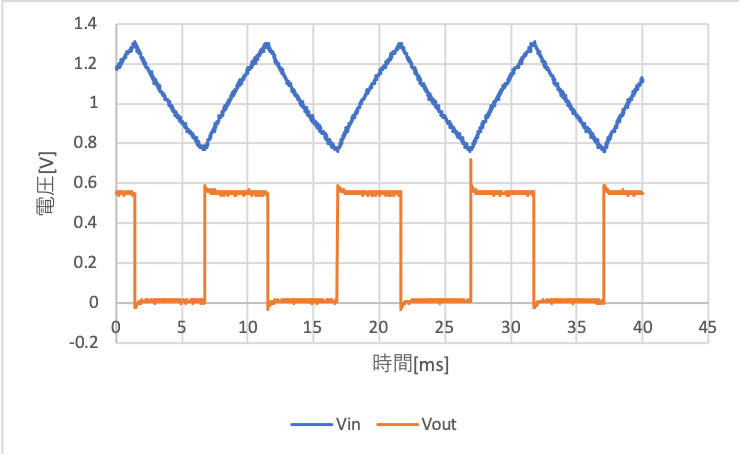
\includegraphics[width=0.8\linewidth]{fig17.png}
 \end{center}
 \caption{W}
 \label{fig:17}
\end{figure}

\begin{figure}[htbp]
 \begin{center}
  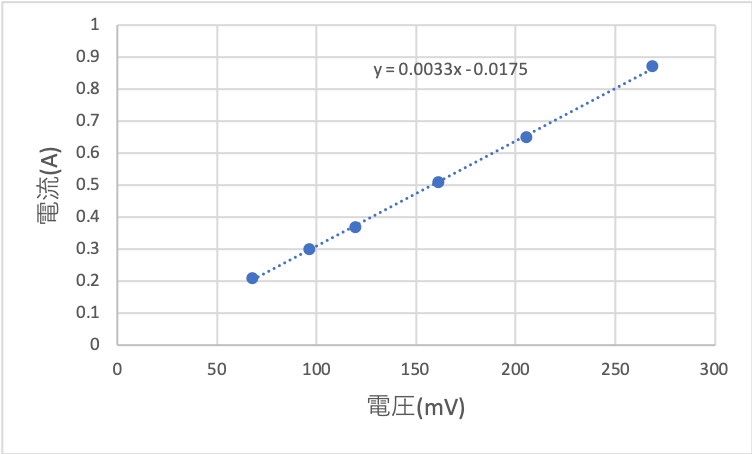
\includegraphics[width=0.8\linewidth]{fig18.png}
 \end{center}
 \caption{シャープペンシルの芯H}
 \label{fig:18}
\end{figure}

\begin{figure}[htbp]
 \begin{center}
  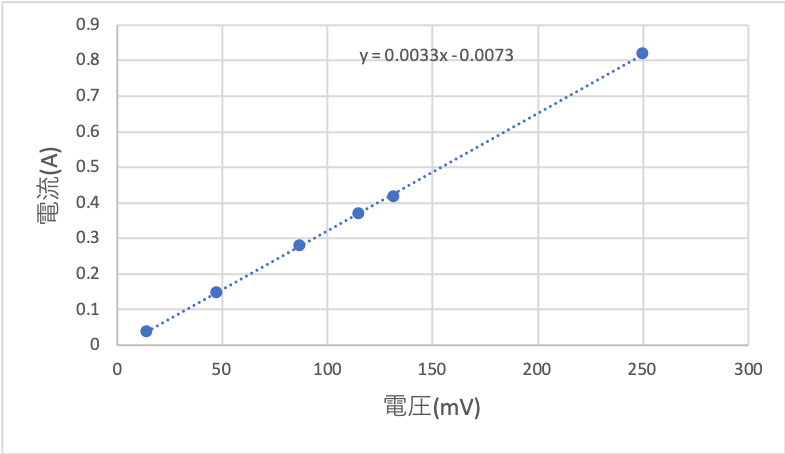
\includegraphics[width=0.8\linewidth]{fig19.png}
 \end{center}
 \caption{シャープペンシルの芯2B}
 \label{fig:19}
\end{figure}

\begin{figure}[htbp]
 \begin{center}
  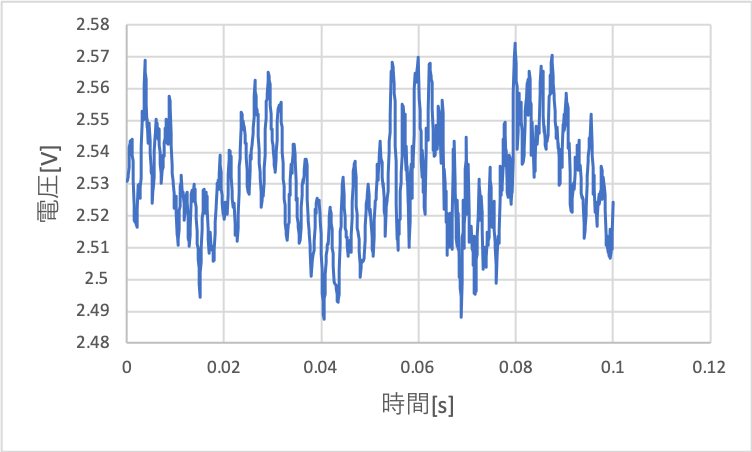
\includegraphics[width=0.8\linewidth]{fig20.png}
 \end{center}
 \caption{Ni}
 \label{fig:20}
\end{figure}

\begin{figure}[htbp]
 \begin{center}
  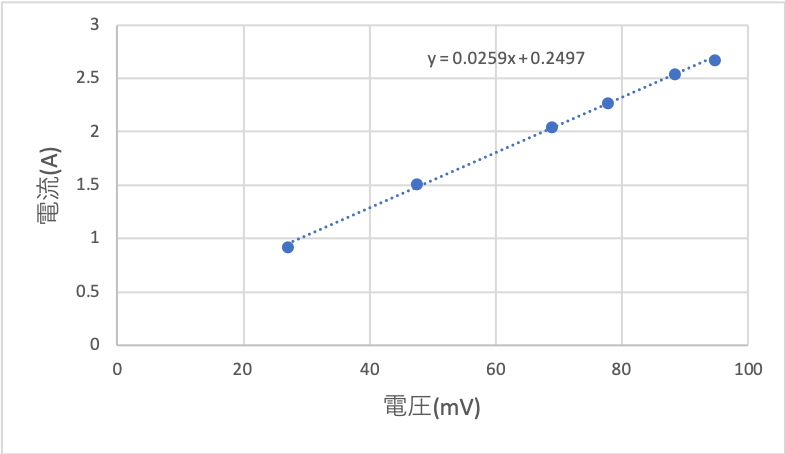
\includegraphics[width=0.8\linewidth]{fig21.png}
 \end{center}
 \caption{Ag}
 \label{fig:21}
\end{figure}

\begin{figure}[htbp]
 \begin{center}
  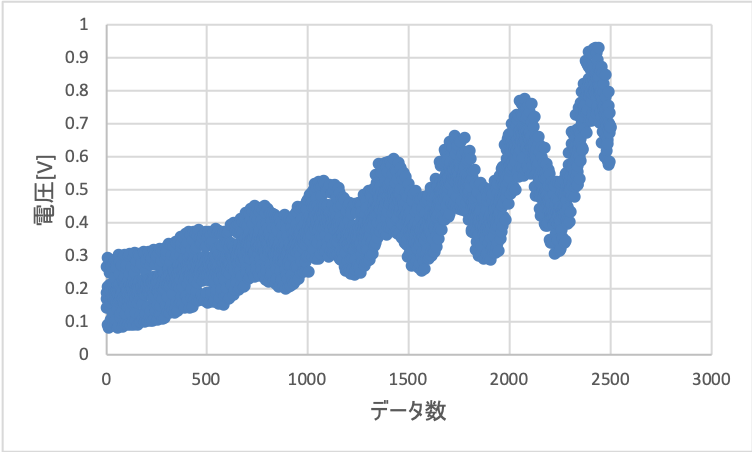
\includegraphics[width=0.8\linewidth]{fig22.png}
 \end{center}
 \caption{不明試料}
 \label{fig:22}
\end{figure}


以上の結果よりグラフの傾きを最小二乗法によって求めそれぞれの抵抗値,抵抗率を求めたところ以下の表のようになった.

\begin{table}[htb]
  \begin{center}
      \caption{抵抗値,抵抗率}
        \begin{tabular}{|c|c|c|} \hline
             試料(直径mm) & 抵抗値($\Omega$) & 2端子($\mu\Omega$cm) \\ \hline
             Cu(0.18) & 0.0132 & 3.35 \\
             NiCr(0.17) & 0.556 & 126 \\
             W(0.09) & 0.1667 & 10.6 \\
             \begin{tabular}{c}
                シャープペンシル \\ の芯H(0.5)
             \end{tabular}
             & 0.3030 & 594 \\
            \begin{tabular}{c}
                シャープペンシル \\ の芯2B(0.5)
            \end{tabular}
             & 0.3030 & 594 \\
             Ni(0.9) & 0.0711 & 45.2 \\
             Ag(0.07) & 0.0386 & 1.49 \\
             不明(0.195) & 0.0735 & 22.0 \\ \hline
        \end{tabular}
  \end{center}
\end{table}

\subsection{Discussion}
どの試料金属においても温度が上昇するにつれて低効率が高くなった現象について考察する.
まず金属はエネルギーバンド図において伝導体に電子を常に持っておりこれは自由電子として電流を運ぶ役割を果たしている.
ここで温度が上昇した場合は格子が熱でより激しく振動することになると予想される.
したがって電子の通り道を格子が塞ぐ確率が高まり結果として単位時間に電子が衝突する回数が多くなり抵抗率が温度の上昇とともに上昇していくと考えられる.
またこの現象から,電子の量が多くなることにより格子に衝突する電子の量が多くなることが予測される.
これはオームの法則の説明であると考えられる.

また測定結果より未知試料だと思われる物質はストロンチウムだと考えられる.
しかし他の金属試料において抵抗率のオーダーはあっているもののその値は理科年表の値から多少ずれており測定において接触抵抗などのノイズが入ったことが考えられる.

またシャープペンシルの芯は濃さに寄らず同じ値を示したことから濃さに寄らずに同じ構造をしていることが予想される.またシャープペンシルの芯はグラフェンであり結合に余分な価電子によって電流を通すが自由電子の数は金属に比べ少ないことが結果から考えられる.
%=============================================================
\newpage
\end{document}

\documentclass[11pt, a4paper,twocolumn]{jarticle}
\usepackage[dvipdfmx]{graphicx}
\usepackage{listings,jlisting}

\begin{document}
%=============================================================
\section{To understand the current-voltage characteristic of semiconductor diodes($3^{rd} day$)}

\subsection{Purpose}
半導体の電流電圧特性を理解する.
\subsection{Procedure}
Siベースダイオード,LED,ツェナーダイオードの三種類の資料について電流電圧特性を計測する.
この時電流が40mAを超えないように注意する.
またヒステリシス特性を観察するために電圧を上昇させた場合と下降させて行った場合の2通りを2回ずつ測定した.

\subsection{Result}
測定の結果電流電圧の関係をプロットすると以下のようなグラフが得られた.
グラフよりいずれのダイオードもある一定の電圧がかからなければ電流を通さない性質を示した.

LEDについては電流が流れるのと同時に発光し始め,電圧を高くするにつれて光は強くなっていった.またいずれのダイオードも逆方向に電圧をかけても電流は流れなかった.

さらにグラフよりわかるように電圧をあげていった場合も電圧を下げた場合も電流の値は同じ値を取ったためヒステリシス特性は示さなかった.

\begin{figure}[htbp]
 \begin{center}
  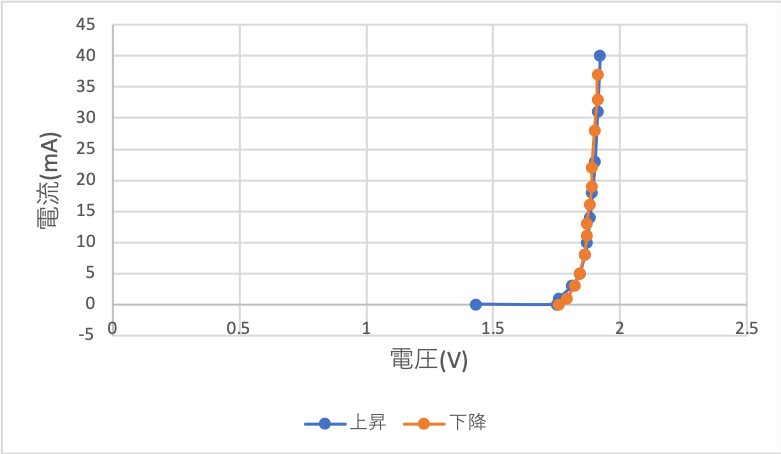
\includegraphics[width=0.8\linewidth]{fig23.png}
 \end{center}
 \caption{LED 1回目}
 \label{fig:23}
\end{figure}

\begin{figure}[htbp]
 \begin{center}
  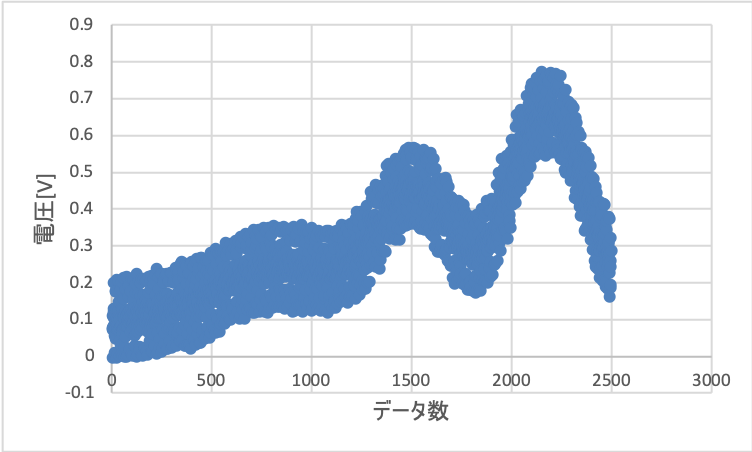
\includegraphics[width=0.8\linewidth]{fig24.png}
 \end{center}
 \caption{LED 2回目}
 \label{fig:24}
\end{figure}

\begin{figure}[htbp]
 \begin{center}
  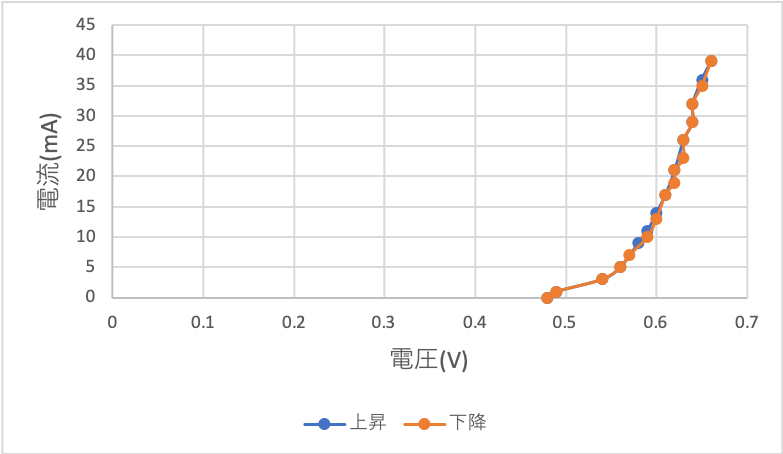
\includegraphics[width=0.8\linewidth]{fig25.png}
 \end{center}
 \caption{Siダイオード 1回目}
 \label{fig:25}
\end{figure}

\begin{figure}[htbp]
 \begin{center}
  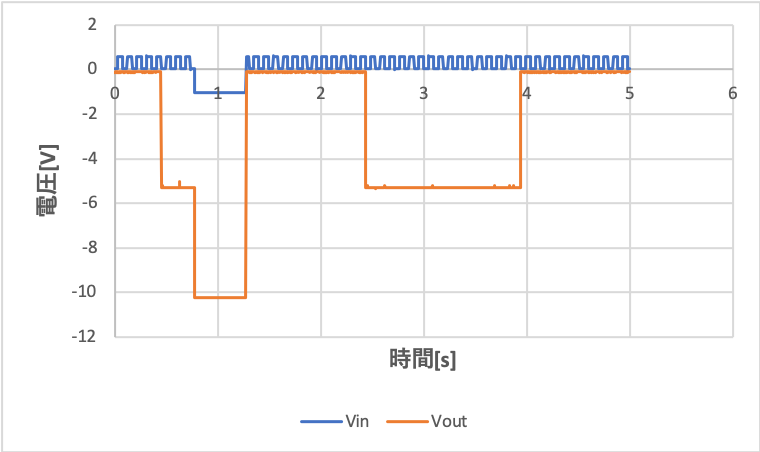
\includegraphics[width=0.8\linewidth]{fig26.png}
 \end{center}
 \caption{Siダイオード 2回目}
 \label{fig:26}
\end{figure}

\newpage

\begin{figure}[htbp]
 \begin{center}
  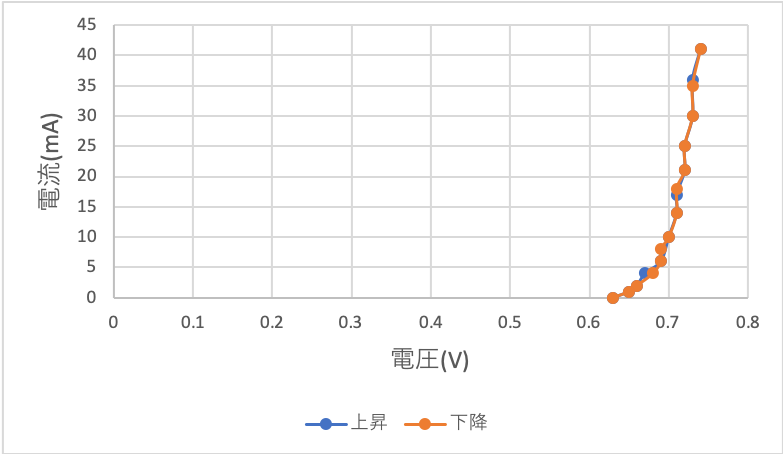
\includegraphics[width=0.8\linewidth]{fig27.png}
 \end{center}
 \caption{ツェナーダイオード 1回目}
 \label{fig:27}
\end{figure}

\begin{figure}[htbp]
 \begin{center}
  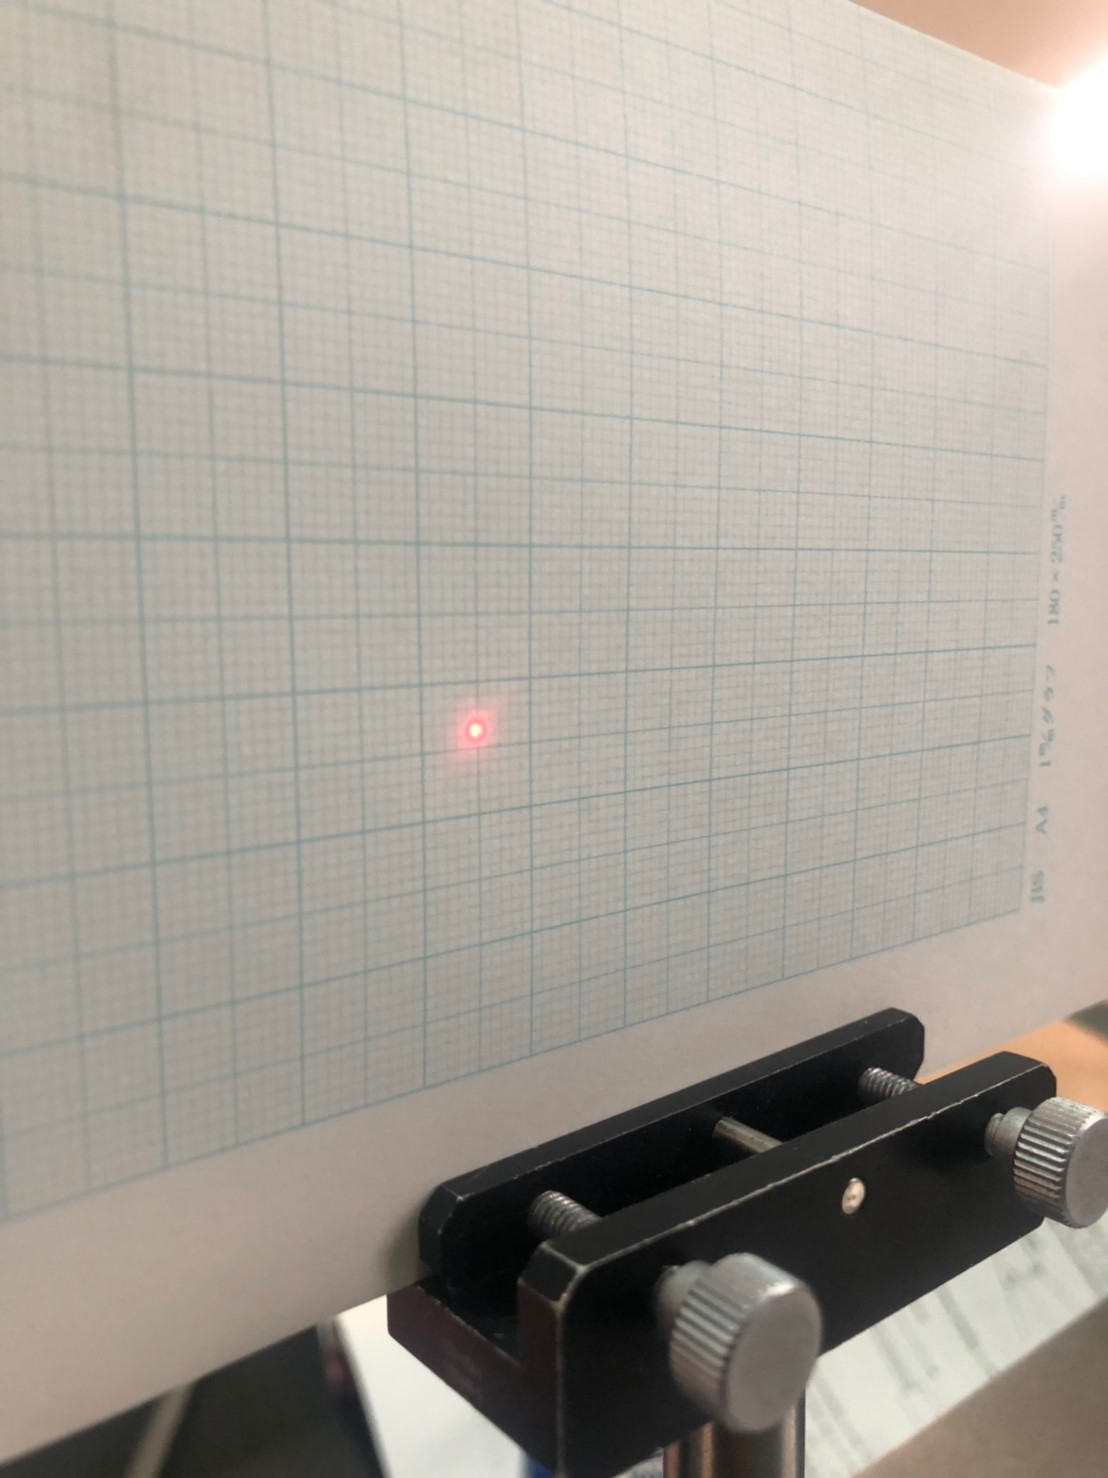
\includegraphics[width=0.8\linewidth]{fig28.png}
 \end{center}
 \caption{ツェナーダイオード 2回目}
 \label{fig:28}
\end{figure}



\subsection{Discussion}
実験結果よりダイオードは順バイアス電圧をかけた際には電流を流すが逆バイアス時には電流は流れない整流作用の特性を持つので電流が逆流して欲しくない回路などに組み込んで応用することができると考えられる.

次にダイオードの順バイアス時にある特定の電圧を超えた際に電流を流し始める特性について考察する.
まずPN接合においては図\ref{fig:36}のようにP領域のキャリアとN領域の電子がそれぞれ接触し消滅する空乏層が生成される.
この空乏層が障壁となるため順バイアスを印加した際にある一定電圧を超えないと電流を流さないのはこの電位障壁が理由だと考えられる.
また逆バイアスをかけた際は空乏層を広げることとなりこの時は電流を流すことはなくなる.これが整流作用の原理だと考えられる.

また逆バイアスをさらに印加していった際の振る舞いについて考察する.
非常に大きな電圧を逆バイアスに印加した際はN型半導体の領域において電子は非常に大きな運動エネルギーを持つことになるがこの運動エネルギーが振動する格子に衝突することで減少し,格子にエネルギーが受け渡されるがこのエネルギーが格子の電子を励起させるのに十分な運動エネルギーを持っていた場合,ぶつかった格子から新たに自由電子とホールのペアが生成される.
またこの反応が再帰的に起こることで急激に電流が流れることが予想される.
今回は実験の時間により逆バイアスの測定ができなかったが図\ref{fig:37}のように電圧電流特性を示すことが予想される.



\begin{figure}[htbp]
 \begin{center}
  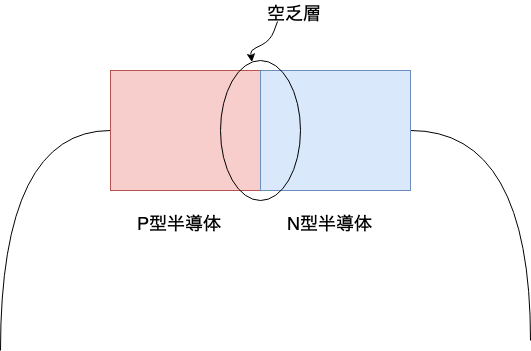
\includegraphics[width=0.8\linewidth]{fig36.png}
 \end{center}
 \caption{PN接合}
 \label{fig:36}
\end{figure}

\begin{figure}[htbp]
 \begin{center}
  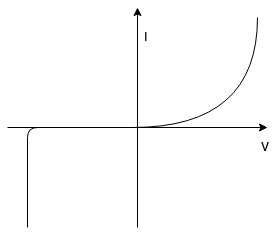
\includegraphics[width=0.8\linewidth]{fig37.png}
 \end{center}
 \caption{電流電圧特性}
 \label{fig:37}
\end{figure}


%=============================================================
\newpage
\end{document}

\documentclass[11pt, a4paper,twocolumn]{jarticle}
\usepackage[dvipdfmx]{graphicx}
\usepackage{listings,jlisting}

\begin{document}
%=============================================================
\section{Temprature dependence of the resistance($4^{th} day$)}

\subsection{Purpose}
金属抵抗の温度による変化を学ぶ.
\subsection{Procedure}
まず試料を四端子測定法の測定回路に接続する.次に熱電対と共に試料を固定し液体窒素の入った容器の中に沈めていく.
この時試料の温度は熱電対の起電力によって測定する.
今回使用した熱電対はクロメルーアルメル熱電対であり測定部分を氷水の容器に浸し基準を273Kにして測定する.
測定器の製作は図\ref{fig:29}のように組み立てる.

以上の手順でCu,NiCr,Wの低効率を測定していく.
測定は室温から77K程度まで5段階に分けて測定を行なった.
測定結果より抵抗値を最小二乗法で求めその温度依存性をグラフに示す.

\begin{figure}[htbp]
 \begin{center}
  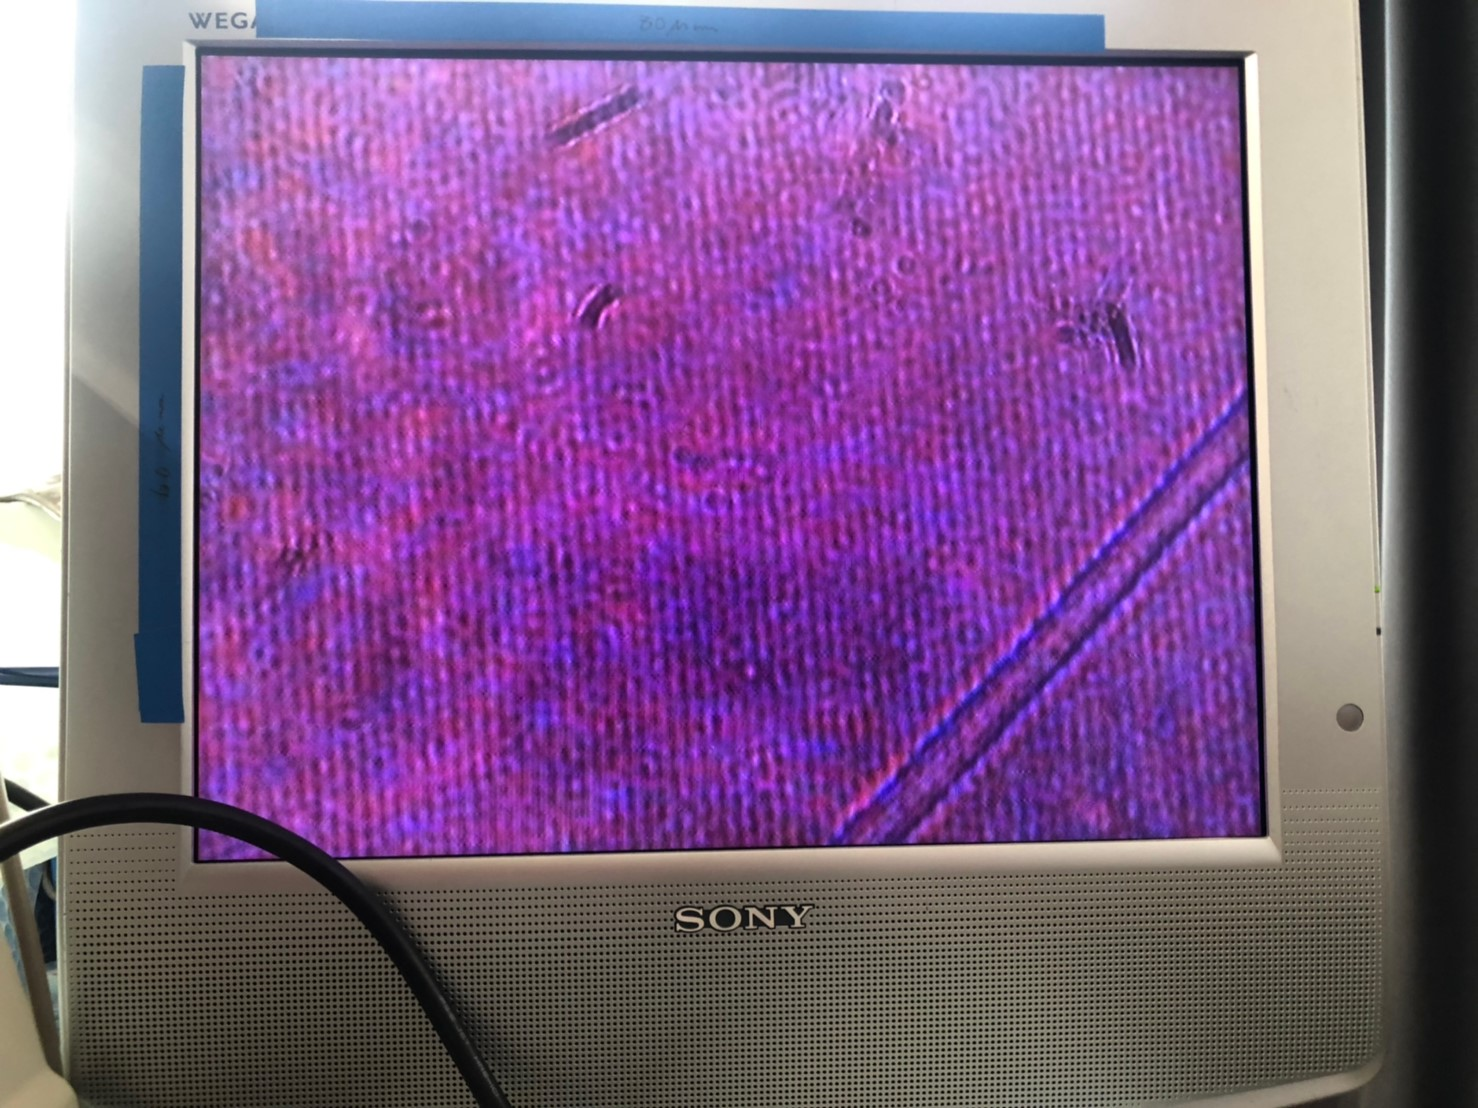
\includegraphics[width=0.8\linewidth]{fig29.png}
 \end{center}
 \caption{温度依存性の実験装置}
 \label{fig:29}
\end{figure}

\subsection{Result}
測定の結果温度と抵抗値の関係をプロットすると以下のようなグラフが得られた.

\begin{figure}[htbp]
 \begin{center}
  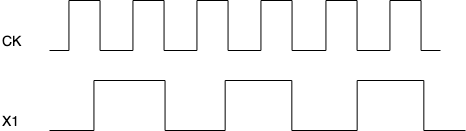
\includegraphics[width=0.8\linewidth]{fig30.png}
 \end{center}
 \caption{Wの温度依存}
 \label{fig:30}
\end{figure}

\begin{figure}[htbp]
 \begin{center}
  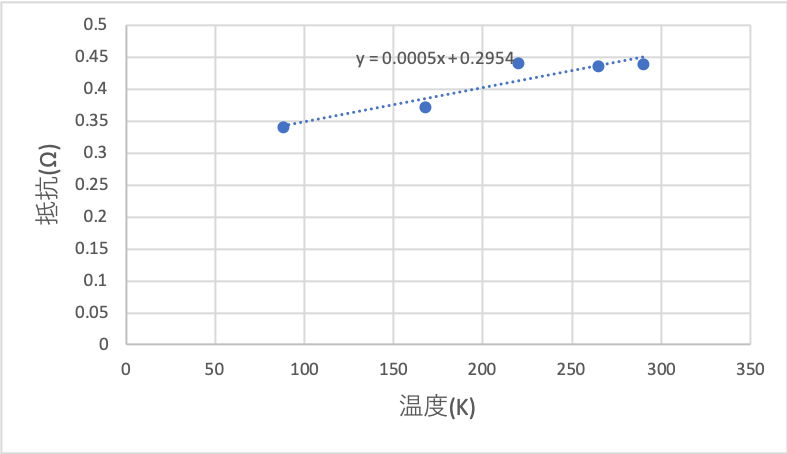
\includegraphics[width=0.8\linewidth]{fig31.png}
 \end{center}
 \caption{NiCrの温度依存}
 \label{fig:31}
\end{figure}

\begin{figure}[htbp]
 \begin{center}
  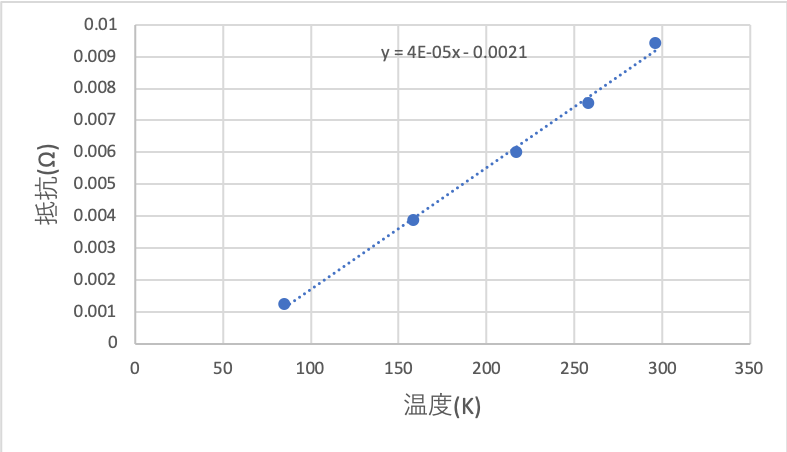
\includegraphics[width=0.8\linewidth]{fig32.png}
 \end{center}
 \caption{Cuの温度依存}
 \label{fig:32}
\end{figure}

\newpage


\subsection{Discussion}
実験結果より温度が低くなるにつれて抵抗率が小さくなった原因について考える.
まず前回の考察より金属中において電流の流れを阻害するものは熱振動する格子だと考えられることがわかった.したがって温度が下がるとその分熱運動により振動する格子の振動の激しさは穏やかになることが予想され結果として電流が格子と衝突する回数がすくなり流れる電流量が多くなり抵抗率が小さくなることが予想される.

%=============================================================
\newpage
\end{document}

\documentclass[11pt, a4paper,twocolumn]{jarticle}
\usepackage[dvipdfmx]{graphicx}
\usepackage{listings,jlisting}

\begin{document}
%=============================================================
\section{Measurement of current-voltage characteristics of thermistor (metal-oxide semiconductor) and mechanical pencil lead(carbon)($5^{th} day$)}

\subsection{Purpose}
サーミスターとシャープペンシルの芯の電気抵抗の温度依存性を学習する.
\subsection{Procedure}
今回はサーミスター(103AT-11)とシャープペンシルの芯(H,2B)について測定をおこなう.
まず前回同様に図\ref{fig:29}のように装置を組み立てて四段階に温度を変えながら測定を行った後,それぞれの抵抗値を電流電圧測定値の傾きを最小二乗法によって求め温度依存性を考察する.

\begin{figure}[htbp]
 \begin{center}
  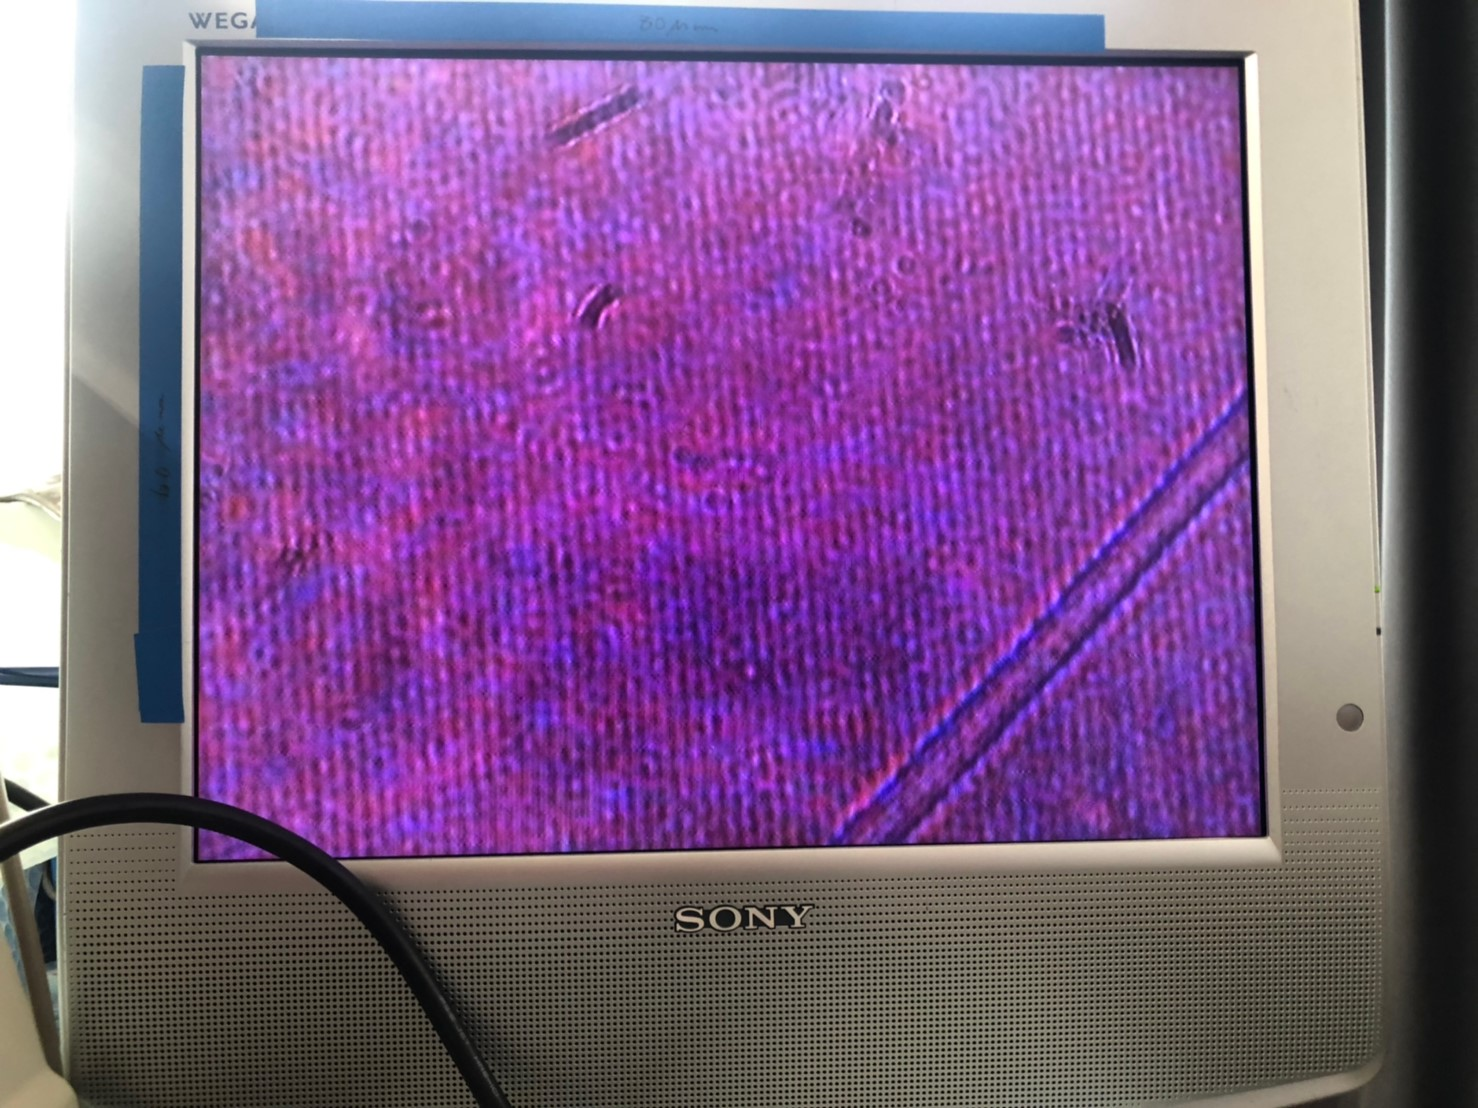
\includegraphics[width=0.8\linewidth]{fig29.png}
 \end{center}
 \caption{温度依存性の実験装置}
 \label{fig:29}
\end{figure}

\subsection{Result}
測定の結果温度と抵抗値の関係をプロットすると以下のようなグラフが得られた.
シャーペンの芯はどちらの芯も同じ温度依存性を示した.
またサーミスターに関しては温度依存性を示さなかった.

\begin{figure}[htbp]
 \begin{center}
  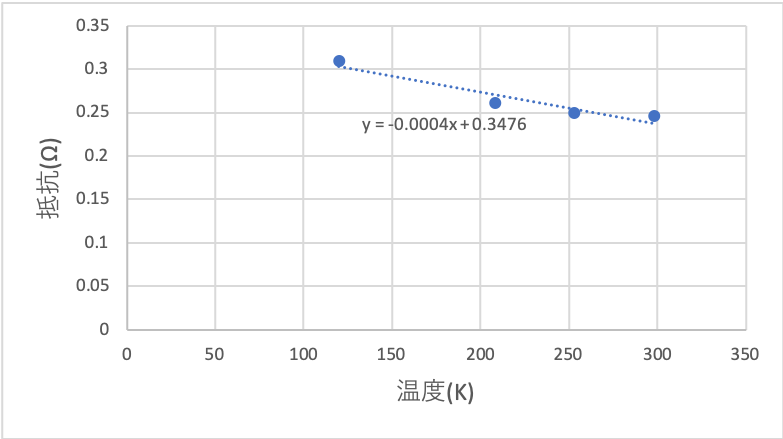
\includegraphics[width=0.8\linewidth]{fig33.png}
 \end{center}
 \caption{カーボン2Bの温度依存}
 \label{fig:33}
\end{figure}

\begin{figure}[htbp]
 \begin{center}
  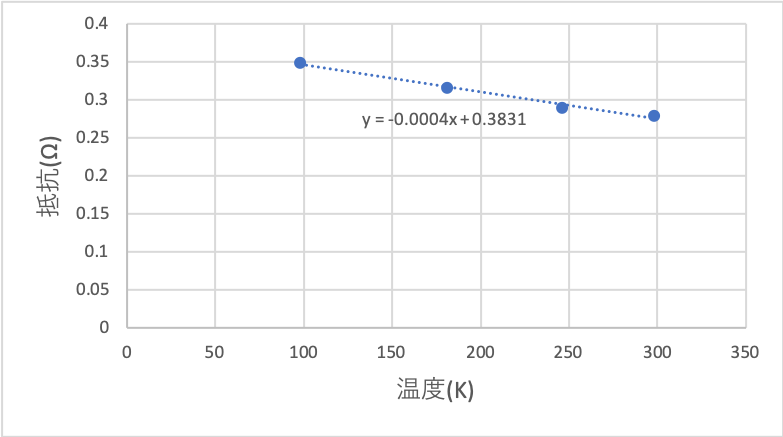
\includegraphics[width=0.8\linewidth]{fig34.png}
 \end{center}
 \caption{カーボンHの温度依存}
 \label{fig:34}
\end{figure}

\begin{figure}[htbp]
 \begin{center}
  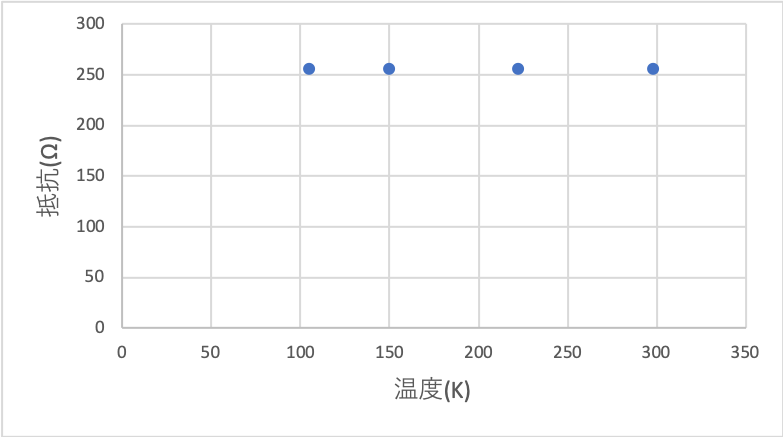
\includegraphics[width=0.8\linewidth]{fig35.png}
 \end{center}
 \caption{サーミスター(103AT-11)の温度依存}
 \label{fig:35}
\end{figure}

\subsection{Discussion}
前回の実験において室温でのシャープペンシルの芯は硬さに関わらず同じ抵抗値を示したのでシャーペンの芯の抵抗特性は硬度に依存しないと考えられたが,今回の実験でもこの二つの硬さにおける測定値に有意な差は観測てできなかったので硬さによってシャープペンシルの芯の構造は変わらないと考えられる.
サーミスターの測定結果より今回の実験ではサーミスターの温度特性を観測できなかったので実験の操作手順をミスしてしまった可能性が考えられる.
もしくはサーミスターの抵抗変化が高温で起こることなどが考えられる.

また今回は前回の金属試料の温度特性と異なり温度が高くなるにつれて抵抗率が低くった原因について考察する.
エネルギーバンド図において非金属の半導体のバンド図は図\ref{fig:37}のようになる.
このバンド図において電子の多くは価電子帯に存在しており伝導体に存在する電子は少量と考えることができる.
温度が上がることにより励起される価電子帯の電子がエネルギーギャップEgを超えることにより伝導帯に存在する電子が増え,結果として抵抗率が小さくなっていくと考えられる.

\begin{figure}[htbp]
 \begin{center}
  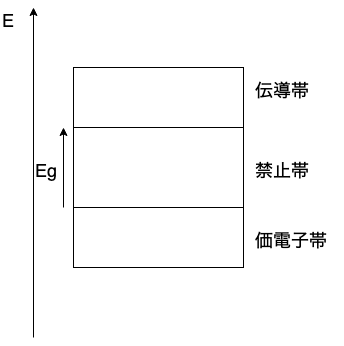
\includegraphics[width=0.8\linewidth]{fig38.png}
 \end{center}
 \caption{半導体のバンド図}
 \label{fig:38}
\end{figure}


%=============================================================
\newpage
\end{document}

\documentclass[11pt, a4paper,twocolumn]{jarticle}
\usepackage[dvipdfmx]{graphicx}
\usepackage{listings,jlisting}

\begin{document}
%=============================================================
\section{Measurement of the temperature dependence of the resistivity of $Bi_2Sr_2Ca_2Cu_3O_{10}$ as a superconductor($6^{th} day$)}

\subsection{Purpose}
超電導の転移温度の測定を通して超電導の原理について学ぶ.
\subsection{Procedure}
前回同様に図\ref{fig:29}のように温度依存性の測定のための実験装置を組み立てる.
次に超電導リボン($Bi_2Sr_2Ca_2Cu_3O_{10}$)の電圧-電流特性を四端子測定法で測定する.
この時超電導のヒステリシス特性を観察するために室温から超電導が起こる相転移温度まで下げていった場合と,超電導状態から室温に近づけていった場合の二パターンについて測定を行いそれぞれの結果を温度-抵抗値のグラフにプロットしていく.
測定の際は電流が100mAを超えないように注意して行う.

\subsection{Result}
測定の結果温度と抵抗値の関係をプロットすると以下のようなグラフが得られた.
ヒステリシスが測定され,室温から温度を下げていった場合よりも超電導状態から室温にあげていった時は結果が全体的に左にシフトした.
また実験結果より温度下降時は相転移温度は140Kほど,上昇時は130Kほどであることが確認された.

\begin{figure}[htbp]
 \begin{center}
  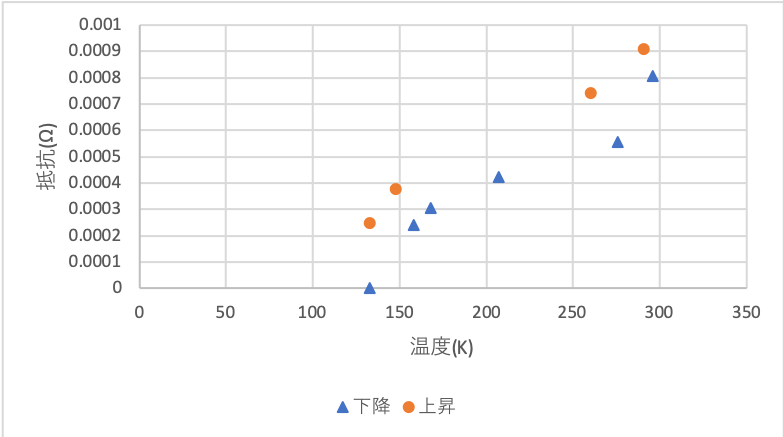
\includegraphics[width=0.8\linewidth]{fig39.png}
 \end{center}
 \caption{温度下降}
 \label{fig:39}
\end{figure}

\subsection{Discussion}
超電導が起こる理由について考える.
まず超電導が起きる極低温状態においては原子の熱振動は十分小さくなっていることが予想される.そこで一つの電子が原子に衝突すると原子が動かされ,プラスに帯電している原子は別の電子を引き寄せるという原理によって結果として電子同士が引き寄せられる現象が図\ref{fig:40}が起きる.
以上のようにして電子のペアについて片方が原子に衝突しても,その衝撃を片方がプラス,もう一方がマイナスに分散吸収してペア全体としては何事もなかったように進むことによって抵抗を感じずに電流を流すことができる.

次に超電導の応用について考える.
超電導状態では小さい電圧で多くの電流を流すことができるので非常に強い磁場を作り出すことが可能である.これはリニアモーターカーなどで利用される.
また量子コンピュータにおいては量子状態がノイズによって壊れることが問題であるためノイズを小さくするために超電導状態が用いられる.
もし超電導状態を室温で実現することができればリニアモータカーが新幹線よりもコストの低い乗り物になることができ,量子コンピュータの製作コストが格段に低くなることが予想される.

\begin{figure}[htbp]
 \begin{center}
  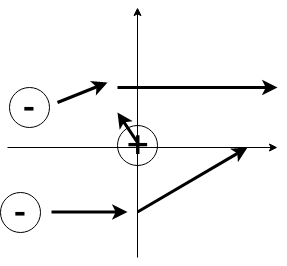
\includegraphics[width=0.8\linewidth]{fig40.png}
 \end{center}
 \caption{超電導メカニズム}
 \label{fig:40}
\end{figure}
%=============================================================
\newpage
\end{document}

%=============================================================
\begin{thebibliography}{9}
  \bibitem{1} 石飛 秀和 他 「応用物理学実験」
  \bibitem{2} 国立天文台  「理科年表」
  \bibitem{3} 小原 実 他 「レーザー応用光学」
  \bibitem{4} 櫛田 孝司  「光物理学」 
\end{thebibliography}
%=============================================================
\end{document}
